\documentclass{article}
\usepackage{graphicx, subfig, fancyhdr, amsmath, amssymb, amsthm, url, hyperref, geometry, listings, xcolor}
\usepackage[utf8]{inputenc}
\usepackage[margin=1in]{geometry}

% Fix Unicode character issues
\DeclareUnicodeCharacter{2212}{-}

\lstset{
    language=C,                         
    basicstyle=\ttfamily\small,         
    numbers=left,                        
    numberstyle=\tiny,                   
    stepnumber=1,                        
    frame=single,                        
    backgroundcolor=\color{gray!10},     
    keywordstyle=\color{blue}\bfseries,  
    commentstyle=\color{green!50!black}, 
    stringstyle=\color{red},             
    breaklines=true,                     
    breakatwhitespace=true,              
    showstringspaces=false,              
    tabsize=4                            
}

\newcommand{\SecondAuthor}{Mohammad Hossein Momeni - Std ID: 99102359}
\newcommand{\FirstAuthor}{Mohammad Parsa Dini - Std ID: 400101204}
\newcommand{\exerciseset}{LAB 6: DTMF Decoder}

\fancypagestyle{plain}{}
\pagestyle{fancy}
\fancyhf{}
\fancyhead[RO,LE]{\sffamily\bfseries\large Sharif University of Technology}
\fancyhead[LO,RE]{\sffamily\bfseries\large EE 25-703: Digital Signal Processing}
\fancyfoot[LO,RE]{\sffamily\bfseries\large LAB 6 Report}
\fancyfoot[RO,LE]{\sffamily\bfseries\thepage}
\renewcommand{\headrulewidth}{1pt}
\renewcommand{\footrulewidth}{1pt}

\graphicspath{{figures/}}

\title{
    \includegraphics[width=3cm]{logo.png} \\ 
    Digital Signal Processing LAB \\ \exerciseset
}
\author{\FirstAuthor \\ \SecondAuthor}
\date{May 2025}

\begin{document}
\maketitle

\section*{Introduction}
This laboratory session focused on implementing a Dual-Tone Multi-Frequency (DTMF) decoder on a DSP development board. The objective was to detect keypad button presses by analyzing audio tones in real-time using interrupt-driven signal processing. Each DTMF key generates a unique combination of two sinusoidal frequencies: one from a low-frequency group (697, 770, 852, 941 Hz) and one from a high-frequency group (1209, 1336, 1477 Hz). The system processes incoming audio signals, identifies the dominant frequencies using matched filtering, and activates corresponding LEDs to indicate the detected key.

\section*{Implementation}

We configured the DSP board and set the input source to the microphone. Using the \texttt{hook\_int()} function, we disabled global interrupts, enabled non-maskable interrupts for critical signals, mapped the serial port receive interrupt to line 15, and activated it for new audio data arrivals.

The \texttt{serialPortRcvISR()} function managed the interrupt service routine by reading incoming audio samples from the codec, amplifying them with a gain factor, and sending the amplified signal to the output. Additionally, it maintained a buffer of size 100 and updated the frame of input data upon each interrupt. Once 50 new samples (determined by a counter) were collected, the processing function was invoked to detect if a DTMF (Dual Tone Multi-Frequency) tone was present in the frame.

We also generated a DTMF signal using MATLAB and tested it successfully. Moreover, we verified the correctness of our implementation by playing DTMF tones from the phone dial pad and confirming that the correct LED lights were triggered in response. This demonstrated that our DTMF detection system was functioning reliably under real conditions.

\begin{lstlisting}
int main(){
    MBZIO_init(DSK6416_AIC23_FREQ_8KHZ); // Initialize DSP system at 8 kHz sample rate
    MBZIO_set_inputsource_microphone();  // Set input source to microphone

    counter = 0;                         // Reset sample counter
    //volumeGain = 3;                   // (Commented out) Set the volume gain factor

    hook_int();                          // Configure and enable interrupts

    while(1){ }                          // Infinite loop (processor waits for interrupts)
}
\end{lstlisting}

We also used this line of code since our microphone is not stereo but the handsfrees are stereo, so we masked half of the 32 bits in order to determine which of the MSB and LSB corresponds to which handsfree. We found that the MSB corresponds to the left handsfree. We also set a Gel file gain in order to adjust the volume.  
\begin{lstlisting}
    temp = ( temp * volumeGain ) & 0xFF00; 
\end{lstlisting}

\section*{DTMF Signal Visualization}
In order to better understand the characteristics of a DTMF signal, we plotted it both in the time domain and time-frequency domain using MATLAB. This helped in visualizing the presence of two distinct frequency components for each key press, confirming the dual-tone nature of the signal.

\begin{figure}[h!]
    \centering
    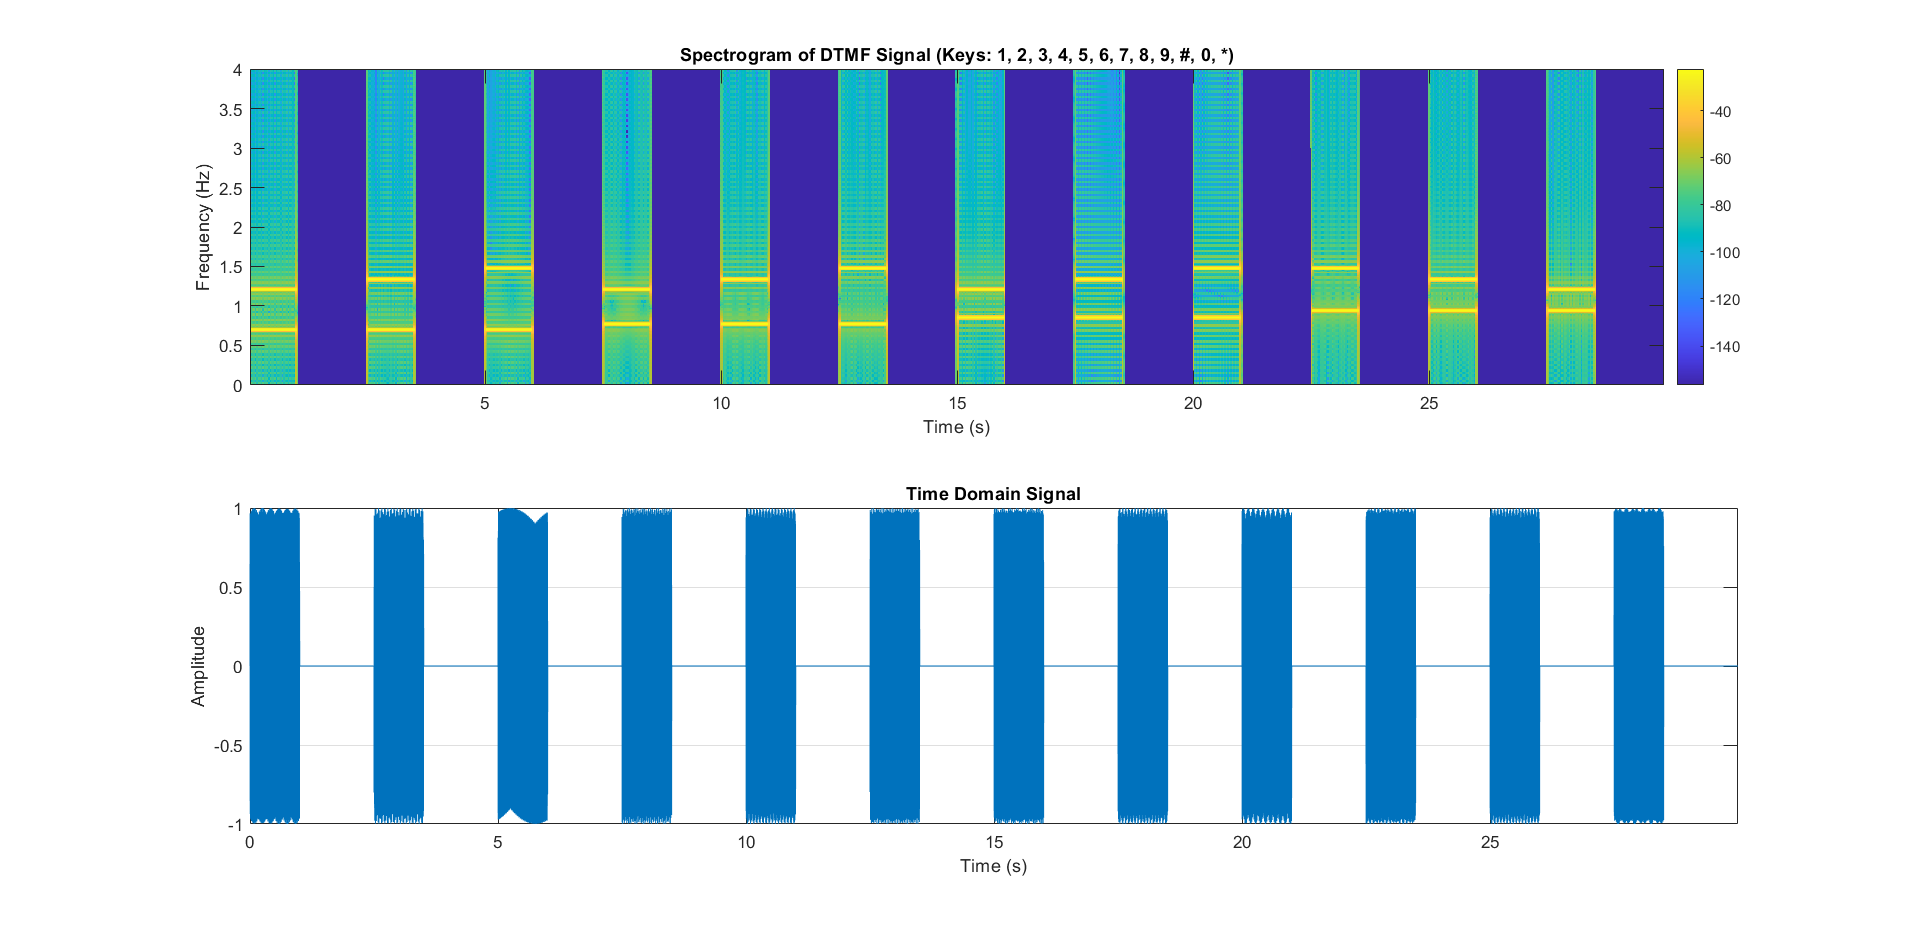
\includegraphics[width=0.8\linewidth]{dtmf.png}
    \caption{DTMF signal in the time domain and its spectogram.}
    \label{fig:dtmf_time}
\end{figure}


\section*{System Overview}
The DTMF decoder operates as follows:
\begin{itemize}
    \item The DSP board is configured to capture audio input via a microphone at a sampling rate of 8 kHz.
    \item Interrupts handle audio sample acquisition,策, avoiding busy waiting.
    \item A sliding buffer of 100 samples stores recent audio data.
    \item Matched filtering, implemented via inner product calculations with sine and cosine components, detects the dominant DTMF frequencies.
    \item The detected frequency pair is mapped to a keypad button.
    \item LEDs on the DSP board are illuminated to indicate the pressed key.
\end{itemize}

\section*{Interrupt Configuration}
The \texttt{hook\_int()} function configures the interrupt system to handle audio input efficiently. It first disables global interrupts to prevent interference during setup. Next, it enables Non-Maskable Interrupts (NMI) to allow high-priority interrupt handling. The function then maps the serial port receive interrupt to line 15, enabling the \texttt{RINT2} interrupt to trigger when new audio data arrives. Finally, global interrupts are re-enabled to resume normal operation. The code is as follows:

\begin{lstlisting}
void hook_int(){
    IRQ_globalDisable();         // Disable global interrupts to prevent interference during setup
    IRQ_nmiEnable();            // Enable Non-Maskable Interrupts for high-priority handling
    IRQ_map(IRQ_EVT_RINT2, 15); // Map serial port receive interrupt to line 15
    IRQ_enable(IRQ_EVT_RINT2);  // Enable RINT2 interrupt for audio data reception
    IRQ_globalEnable();         // Re-enable global interrupts to resume normal operation
}
\end{lstlisting}

\section*{Interrupt Service Routine}
The interrupt service routine (ISR), \texttt{serialPortRcvISR()}, handles real-time audio signal acquisition by reading samples from the codec, amplifying them using \texttt{volumeGain}, and writing the processed output back. It also manages buffering by updating a data frame with each sample and, after collecting 50 new samples, calls the processing function to check for DTMF tone detection.

\begin{lstlisting}
interrupt void serialPortRcvISR(){
    short int buffer_right[100];
    Uint32 temp_right, temp;
    DSK6416_AIC23_read(hCodec, &temp);
    temp_right = (temp * volumeGain) & 0xFFFF;

    for (i=99; i>0; i--) {
        buffer_right[i] = buffer_right[i-1];
    }
    buffer_right[0] = (short int)temp_right;
    counter++;

    if(counter == 100){
        counter = 0;
        processing(buffer_right);
    }
}
\end{lstlisting}

This ISR updates a buffer of 100 samples with the latest audio sample and invokes the \texttt{processing()} function every 100 samples.

\section*{DTMF Signal Processing}
The \texttt{processing()} function performs frequency detection by computing the correlation (inner product) of the input signal with sine and cosine components of each DTMF frequency using the \texttt{max\_inner\_prod()} function. The strongest components—one from the high-frequency group (1209, 1336, 1477 Hz) and one from the low-frequency group (697, 770, 852, 941 Hz)—identify the pressed key.

\textbf{Detection logic:}
\begin{lstlisting}
double max_inner_prod(short int* x, int l, double fc) {
    double sum1 = 0, sum2 = 0;
    for (int i = 0; i < l; i++) {
        sum1 += sin(2 * M_PI * fc * i / Fs) * ((double)x[i]) / 1000;
        sum2 += cos(2 * M_PI * fc * i / Fs) * ((double)x[i]) / 1000;
    }
    return max(abs(sum1), abs(sum2));
}
\end{lstlisting}

The sampling frequency (\texttt{Fs}) is 8000 Hz, and the buffer length (\texttt{l}) is 100 samples. A threshold (\texttt{THR = 1}) ensures robust detection by rejecting weak correlations.

\section*{LED Indication}
The \texttt{LED()} function maps the detected row and column indices to a unique key and activates specific LEDs. If the correlation values fall below the threshold, all LEDs are turned off:

\begin{lstlisting}
void LED(int i, int j){
    index = i + 3*j + 1;
    if (index%2==1){
        DSK6416_LED_on(0);
    } 
    if (index >=8){
        DSK6416_LED_on(3);
        index -= 8;
    } 
    if (index>=4) {
        DSK6416_LED_on(2);
        index -= 4;
    } 
    if (index>=2) {
        DSK6416_LED_on(1);
        index -= 2;
    }
}
\end{lstlisting}

\section*{Conclusion}
This lab demonstrated real-time digital signal processing on embedded hardware using interrupts. The DTMF decoder successfully processed audio inputs, detected frequency components via matched filtering, and indicated key presses using LEDs. The interrupt-driven approach ensured efficient data handling without polling, highlighting a fundamental principle of real-time embedded systems.

\end{document}
